\indent Para estudiar el comportamiento de nuestros algoritmos con distintos tipos de entradas, se generaron 7 familias, cada una con distintas caracter\'isticas, las cuales nos permitirán evaluár las  podas y estrategias tomadas en los algoritmos. Las mismas son las siguientes:

\begin{enumerate}
\item {\bf Familia 1:}  Sin solución. La capacidad de la mochila no es apta para ganar ciertos gimnasios
\item {\bf Familia 2:} Sin soluci\'on. La cantidad de pokeparadas no es suficiente para ganar todos los gimnasios
\item {\bf Familia 3:} Con solución. Ning\'un gimnasio necesita pociones para ser vencido.
\item {\bf Familia 4:} Con solución. Algún gimnasio necesita pociones para ser vencido y las pociones disponibles son suficientes.
\item {\bf Familia 5:} Con solución. La solución corresponde a ordenar los elementos recibidos por distancia.
\item {\bf Familia 6:} Con solución. Entrada fuera de orden, caso opuesto a la familia 5.
\item {\bf Familia 7:} Con solución. Se busca agrupar los elementos de forma que haya muchas soluciones cercanas a la óptima. Esto se logra formando anillos concentricos de gimnasios y pokeparadas.
\item {\bf Familia 8:} Random.
\end{enumerate}


 \subsubsection*{Ejemplificaciones de las familias}
 
Para las representaciones de los casos se utilizan las siguientes referencias:
\begin{figure} [!ht]
\center
 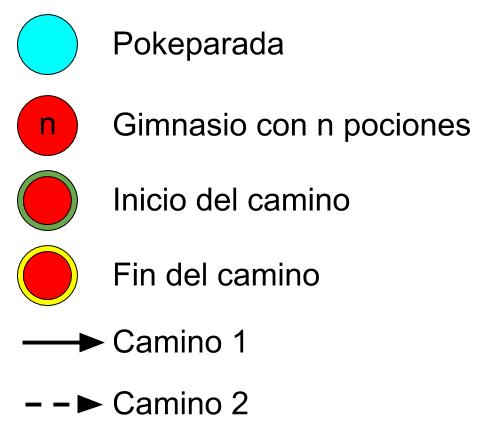
\includegraphics[width=0.30\textwidth]{./EJ1/referencias.jpeg}
\end{figure}
 
\begin{figure} [!ht]
 \centering
  \subfloat[Familia 1: K=3, pociones necesarias = 6]{
    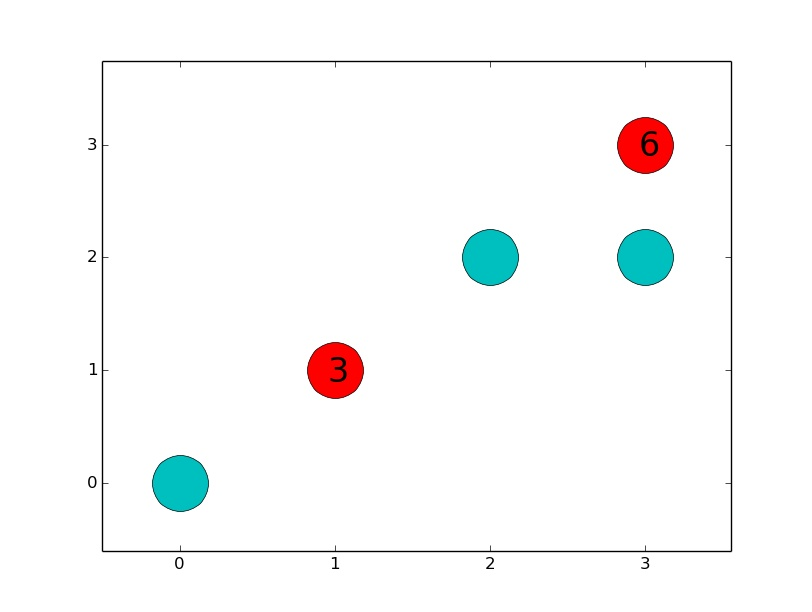
\includegraphics[width=0.40\textwidth]{./EJ1/sinSolucion.jpeg}}
       \label{fig:ss}
  \subfloat[Familia 2: No hay suficientes pociones]{
    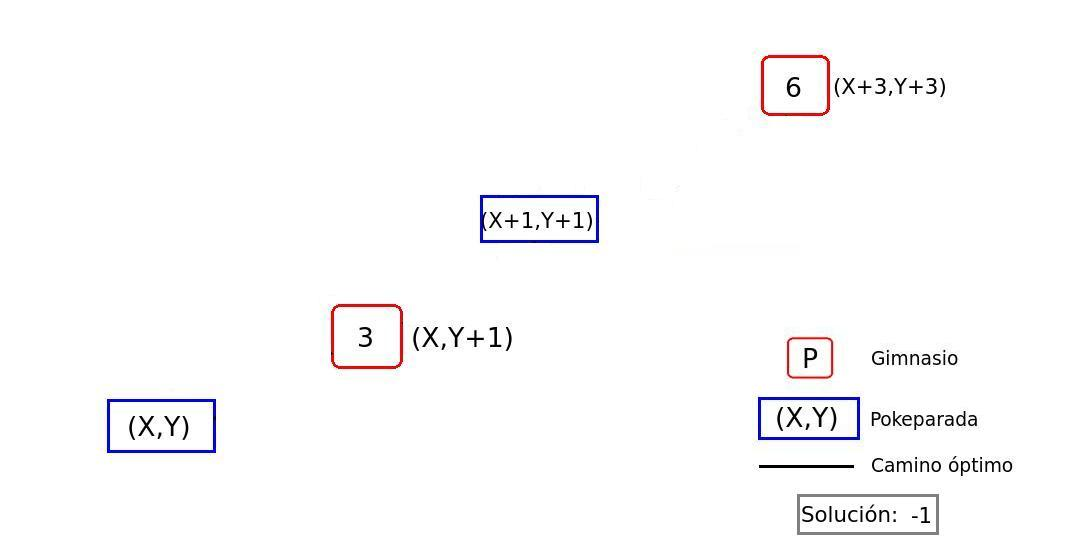
\includegraphics[width=0.40\textwidth]{./EJ1/sinSolucion1.jpeg}}
    \label{fig:ss1}
    \end{figure}\begin{figure} [!ht]
    \centering
     \subfloat[Familia 3: Gimnasios de 0 pociones]{
    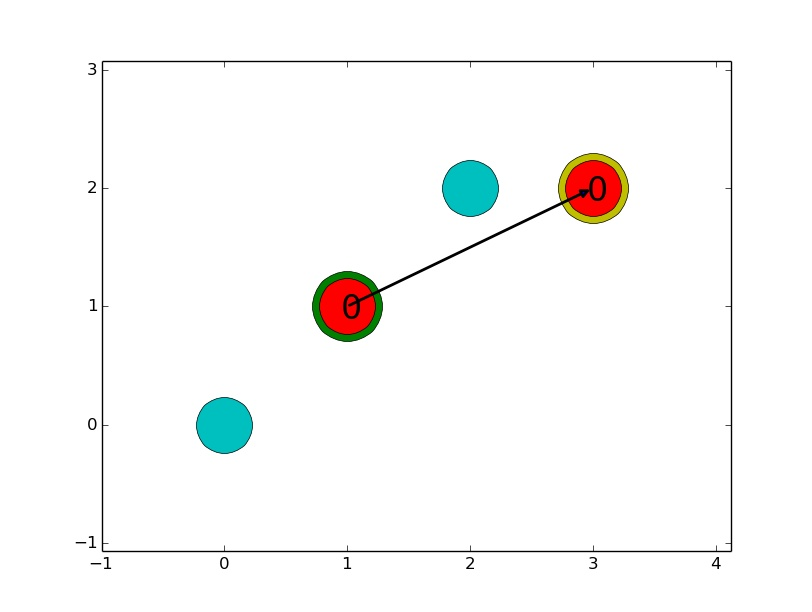
\includegraphics[width=0.40\textwidth]{./EJ1/gym0.jpeg}}
    \label{fig:f3}
 \subfloat[Familia 4: Caso normal]{
    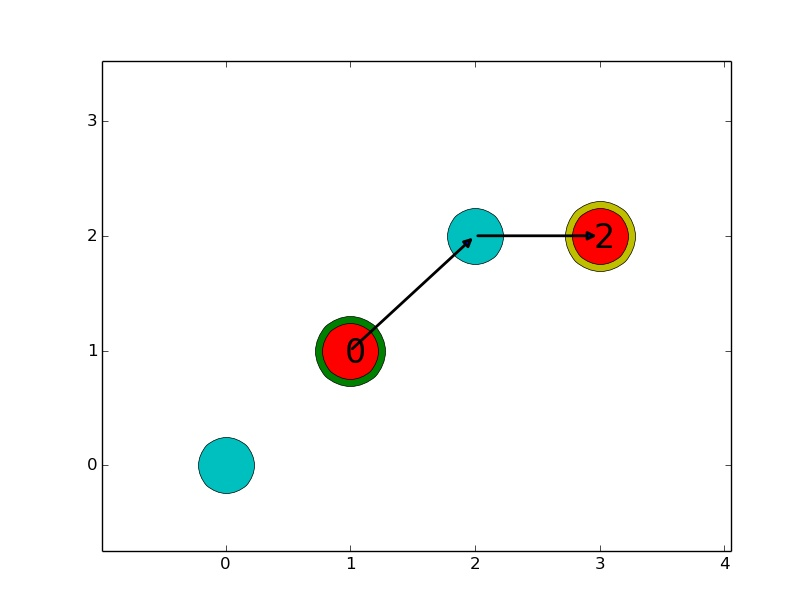
\includegraphics[width=0.40\textwidth]{./EJ1/gymPos.jpeg}}
    \label{fig:f4}
\end{figure}\begin{figure} [!ht]
 \centering
\subfloat[Familia 5: Solución ordenada]{
    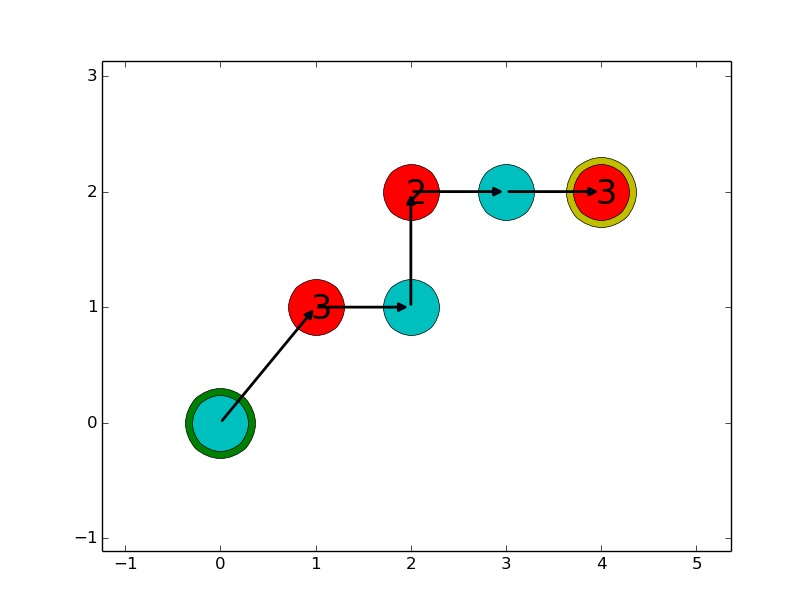
\includegraphics[width=0.40\textwidth]{./EJ1/fam5.jpeg}}
    \label{fig:f5}
\subfloat[Familia 6: Solución desordenada]{
    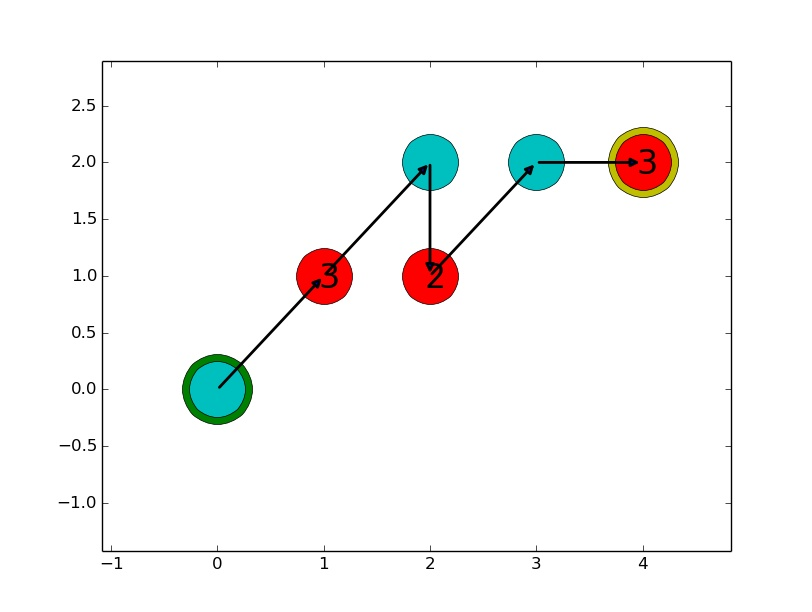
\includegraphics[width=0.40\textwidth]{./EJ1/fam6.jpeg}}
    \label{fig:f6}
\subfloat[Familia 7: Anillos]{
    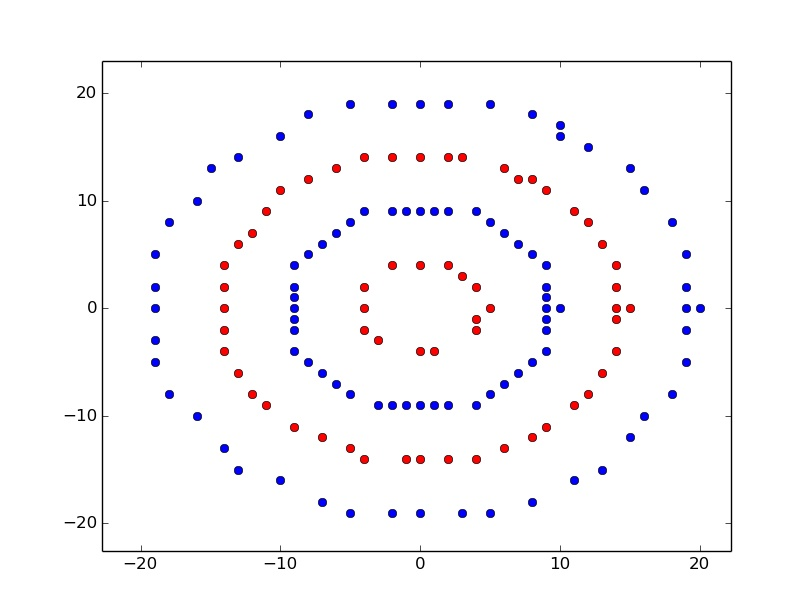
\includegraphics[width=0.40\textwidth]{./EJ1/fam7.jpeg}}
    \label{fig:f7}
\subfloat[Familia 8: Random]{
    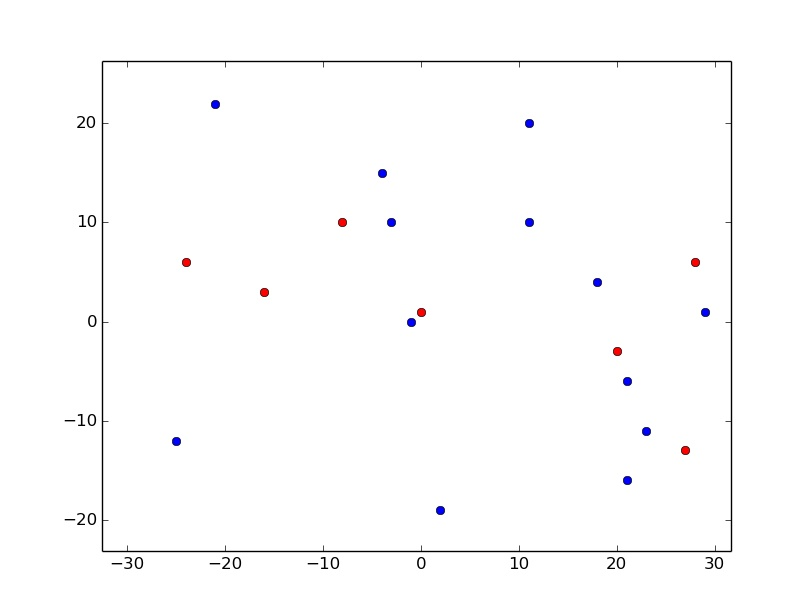
\includegraphics[width=0.40\textwidth]{./EJ1/fam8.jpeg}}
    \label{fig:f8}
\end{figure}


\newpage
 
 
  \subsubsection*{Evaluación del algoritmo sobre las familias}

\indent Veremos entonces que es lo que sucede al ir variando los parámetros de entrada para cada familia, de manera tal que, a medida que N y M crecen linealmente.\\

Se comienza con una entrada de un gimnasio y una pokeparada y se la aumenta en cada test en uno hasta llegar a un total de 20 elementos entre ambos conjuntos (Debido al poder de computo, no es posible trabajar con instancias de mayor tamaño).\\

Para obtener las mediciones se realizaron aproximadamente unas 20 corridas sobre cada una de las instancias y se tom\'o el promedio de las mediciones resultantes.\\ 

Se puede observar en el  gráfico 1.1, ocho funciones, que representan el tiempo de ejecuci\'on de las familias de casos mencionadas en el apartado anterior, utilizando una escala logar\'itmica para una mejor visualizaci\'on de cada funci\'on:\\


\vspace*{0.3cm} \vspace*{0.3cm}
  \begin{center}
 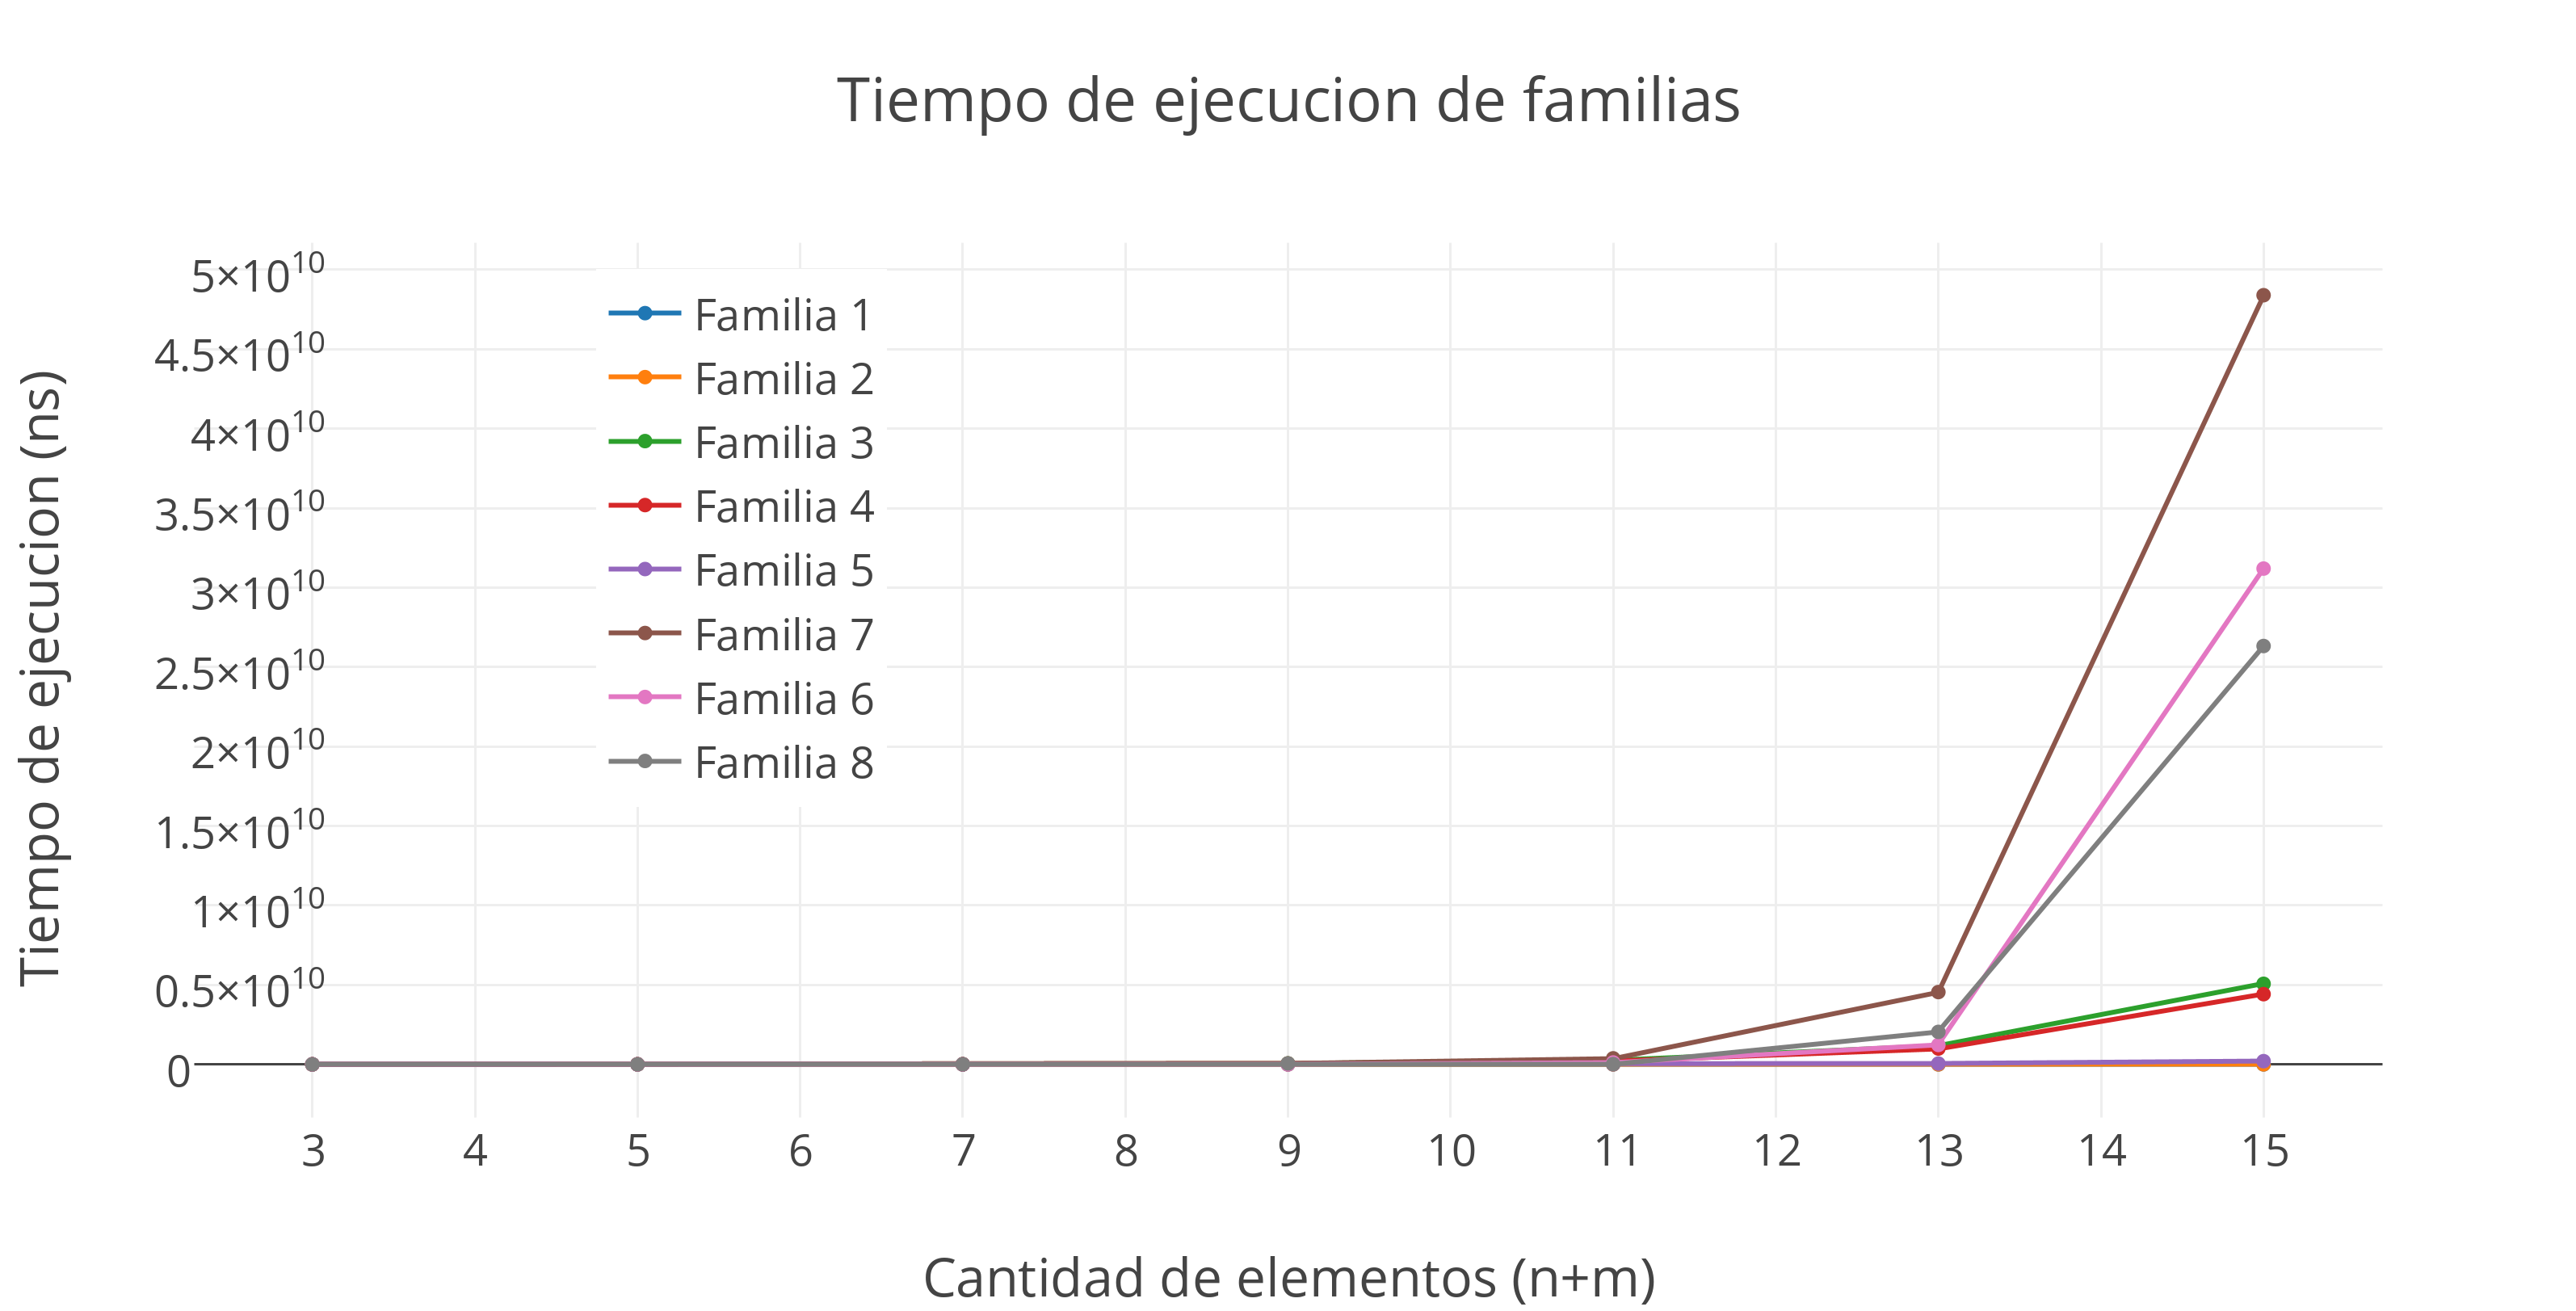
\includegraphics[scale=0.65]{./EJ1/comparativo.png}
 {Gr\'afico \ 1.1 - $Comparativo$}
  \end{center}
  \vspace*{0.3cm}

  
Se puede notar que la familia 1 y la n\'umero 2, presentan una mejor performance en relaci\'on a las otras. Esto se debe a que se realizan dos podas para chequear si la entrada posee o no soluci\'on. Puntualmente, la familia 1 es un poco mejor que la 2 debido a que en la implementaci\'on de las podas, la que evalúa si la mochila es de capacidad suficiente, corta apenas encuentra un gimnasio que no se pueda derrotar. En cambio la otra (chequeo de la cantidad de pociones disponibles vs necesarias) debe necesariamente chequear todos los gimnasios y pokeparadas, tardando más tiempo.

Uno de los peores casos para nuestro algoritmo es la familia 7 , que sucede cuando todos los caminos tienen igual longitud. Esto se da as\'i ya que nuestro algoritmo chequea todas las ramas posibles y, como todas pueden generar una soluci\'on posible, avanza por ellas, llegando al final de cada una con el mismo valor.\\

\vspace*{0.3cm} \vspace*{0.3cm}
  \begin{center}
 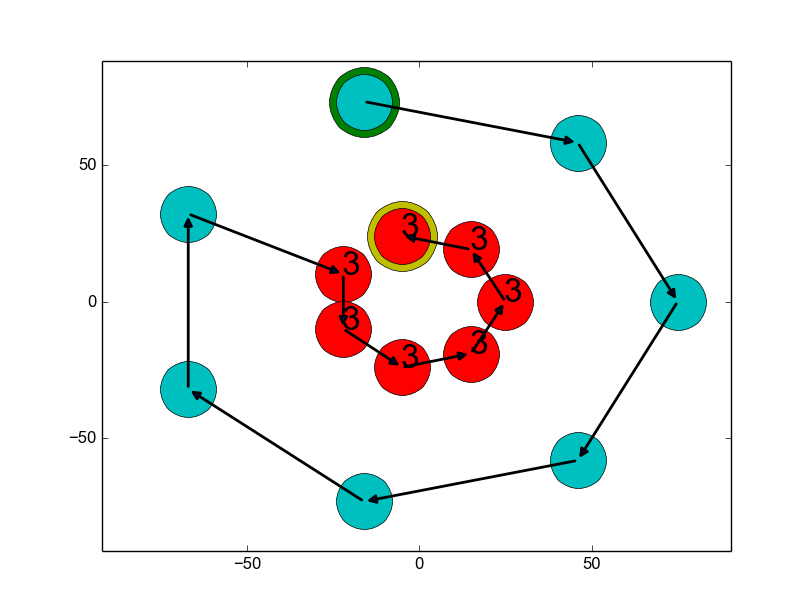
\includegraphics[scale=0.6]{./EJ1/anilloexacto.png}
 {\\Ejemplo n y m iguales en 7 elementos cada uno}
  \end{center}
  \vspace*{0.3cm}


 \subsubsection*{Cota al tiempo de ejecución}


Como se trabaja con pocos casos y la complejidad te\'orica es muy grande, no ser\'a posible graficarla ya que el tiempo insumido es muy elevado, y dado que N+M es pequeño (1 a 20), la muestra no es significativa. De querer trabajar con N+M > 20, la capacidad de cómputo de los dispositivos físicos disponibles es inferior a la necesaria, haciendo impracticable su análisis.



